\documentclass[]{article}

\usepackage[utf8]{inputenc}
\usepackage[french]{babel}
\usepackage{color}

\usepackage{amsmath}
\usepackage{algorithm}
\usepackage{algpseudocode}
\usepackage{frpseudocode}
\renewcommand*\Call[2]{\textproc{#1}(#2)}

\usepackage{url}

\usepackage[left=2.0cm, right=2.0cm, top=2.0cm, bottom=2.0cm]{geometry}

\usepackage[final]{graphicx}[draft]
\graphicspath{{./medias/}}

\usepackage{tikz, pgfplots}
\usetikzlibrary{positioning,fit,arrows.meta}
\usepackage[all]{xy}
\pgfplotsset{compat=1.5}

\title{Implantation Fonctionnelle\\d'Algorithmes Géométriques en 3D\\[0.5cm]
  \large Rapport de projet de recherche\\[0.25cm]Le cas de l'enveloppe convexe : Quickhull}
\author{
	Titouan Laurent - Master 1 parcours Image et 3D\\
	Encadrant : Nicolas Magaud
}
\date{}

\begin{document}

\makeatletter
\begin{titlepage}
	\begin{center}
		{\huge \bfseries  \@title }\\[1cm]
		{\large  \@author}\\[2cm]
		\begin{center}
			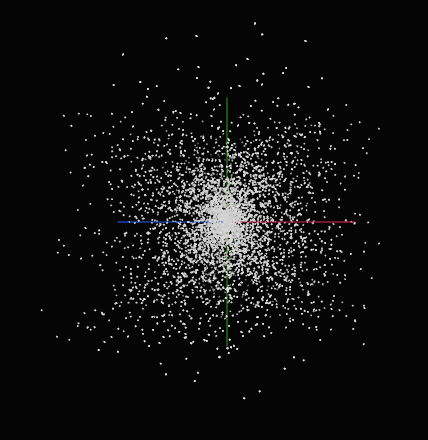
\includegraphics[width=5cm]{illus/illus0.png}
			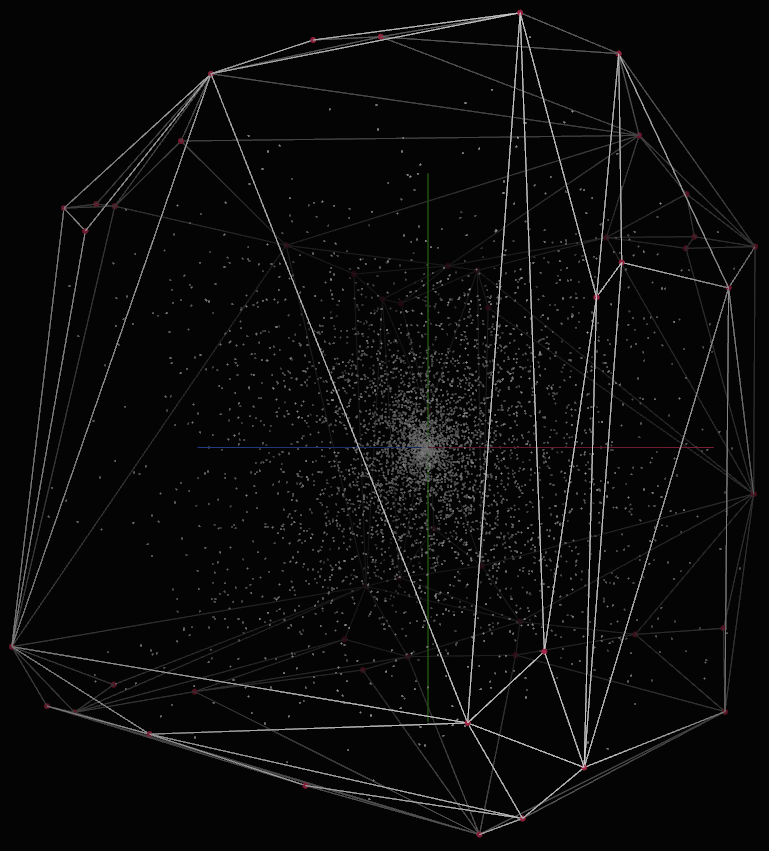
\includegraphics[width=5cm]{illus/illus1.png}
			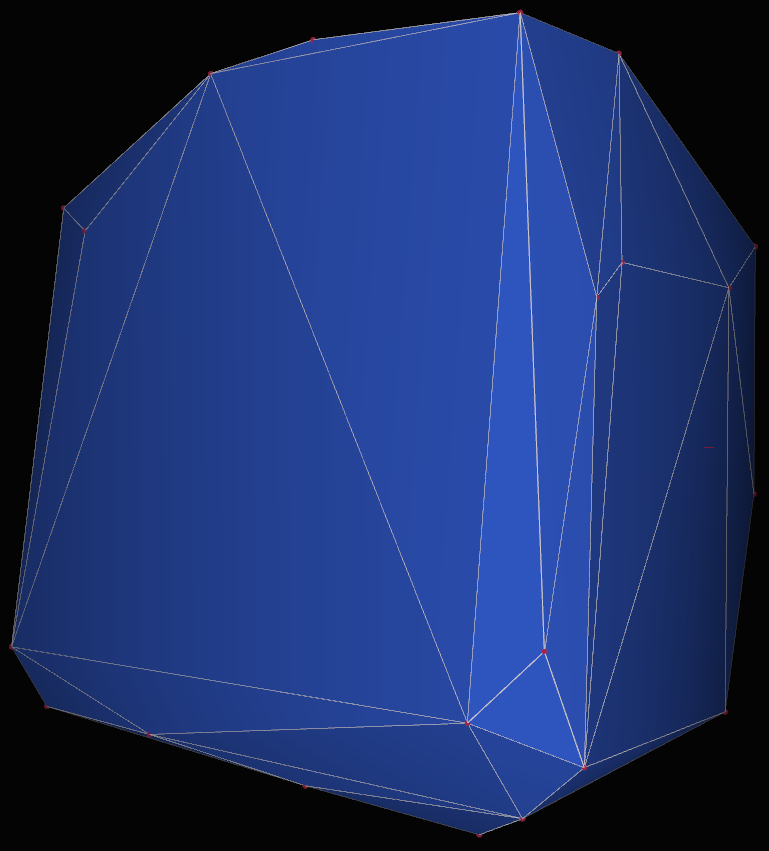
\includegraphics[width=5cm]{illus/illus2.png}
			\\[8cm]
		\end{center}
		
\includegraphics[width=0.15\linewidth]{logos/icube.jpg}
		\hspace{1cm}
		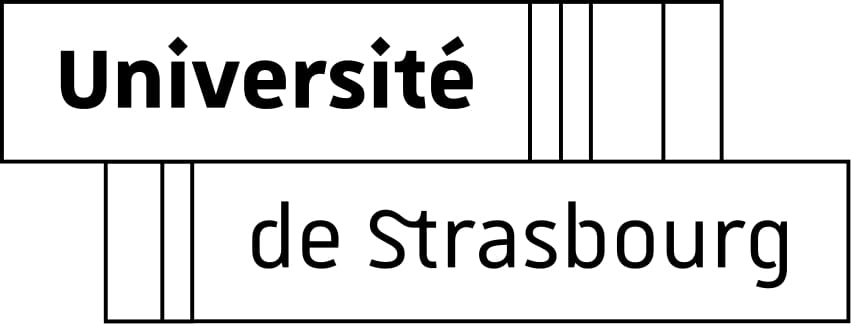
\includegraphics[width=0.2\linewidth]{logos/uds.jpg}
		\\[1cm]
		Note : l'impression couleur est recommandée pour ce document.
	\end{center}
\end{titlepage}
\makeatother

\pagebreak
\tableofcontents

\pagebreak
\section{Introduction}
\paragraph{Preuve assistée par ordinateur}
Prouver la correction d'un algorithme, c'est à dire démontrer formellement qu'il répond à des spécifications précises, est une tâche essentielle dans de nombreux domaines de l'informatique. Cela permet de s'assurer de sa robustesse, et donc, de celle des implantations qui en découlent.

Cependant, il peut être fastidieux de chercher à faire une démonstration formelle à la main, d'autant plus qu'en informatique l'écart entre une implantation donnée et sa description (formelle) représente une limite. Dans le cas des algorithmes géométriques, il y a l'introduction de difficultés supplémentaires, puisque l'on se retrouve généralement à travailler aussi bien sur des notions topologiques qu'arithmétiques.

À partir de là, les outils de preuve automatique se présentent comme une solution viable. Ils permettent de démontrer des propriétés dans une implantation donnée d'un algorithme, et donc d'en prouver la correction. La contrainte étant que, l'implantation doit être faite dans un style de programmation fonctionnel. Leur intérêt réside aussi dans le fait qu'on peut en extraire un programme certifié.

\paragraph{Application au calcul de l'enveloppe convexe}
Le calcul de l'enveloppe convexe d'un ensemble fini de points est un problème bien connu en géométrie et en informatique. Un certain nombre d'algorithmes existent pour le résoudre, et parmi ceux-ci il y a Quickhull, inspiré de Quicksort, qui propose une approche de type \emph{diviser pour régner}, lui assurant une complexité en $O(n\log{n})$.

Par le passé, une implantation incrémentale du calcul de l'enveloppe convexe, restreinte aux ensembles de points à deux dimensions a été proposée et prouvée formellement \cite{brun:hal-00955400, brun:hal-00916880}. On souhaiterait en faire de même avec Quickhull, mais en trois dimensions. Ce n'est pas une tâche triviale, notamment à cause de contraintes supplémentaires de visibilité — qu'on ne retrouve pas en deux dimensions. Il faut également ajouter que les implantations en trois dimensions existantes sont, pour la grande majorité, faites dans un style de programmation impératif, et donc pas directement adaptées à la formalisation dans un assistant de preuves comme Coq \cite{coqref, casteran:hal-00344237}.

\paragraph{}
Mon travail de recherche a donc pour objectif d'explorer ce qui est envisageable en terme d'implantation en style de programmation fonctionnel, mais aussi d'aide à la visualisation de l'algorithme Quickhull en trois dimensions. La finalité étant de pouvoir en faire la démonstration formelle avec Coq.

\section{Choix d'un langage de programmation}
Pour ce sujet, le langage de programmation retenu est celui de Coq. Coq est un assistant à la construction de preuves, codées avec une syntaxe qui lui est propre, en paradigme fonctionnel.

Seulement, ici il présente au moins quatre limitations importantes :
\begin{itemize}
	\item C'est un langage plutôt austère à prendre en main, sa syntaxe est loin d'être évidente et donc il n'est que peu pratique pour développer rapidement et aisément.
	\item Il ne permet nativement pas de faire du dessin graphique, ce qui serait pourtant très pratique pour vérifier visuellement le bon fonctionnement des programmes développés.
	\item Il en est de même pour la lecture et l'écriture de fichiers (par exemple, pour stocker l'enveloppe convexe).
	\item Coq n'est pas un environnement dédié à l'exécution de programmes. En effet, il n'est que très peu performant en temps et en capacités de calcul, même lorsqu'il s'agit de faire des opérations arithmétiques sur de simples entiers non signés.
\end{itemize}

\subparagraph{}
J'ai donc porté mon choix sur le \textbf{JavaScript}, et ce pour les raisons suivantes :
\begin{itemize}
	\item Mis à part Coq, je n'ai jamais utilisé de langage purement fonctionnel jusque-là.
	\item Hors, JavaScript, un langage que je connais particulièrement bien, est \textbf{multi-paradigme}, et donc il permet nativement de développer dans un style de \textbf{programmation fonctionnel}.
	\item JavaScript est adapté à la lecture/écriture de fichiers.
	\item JavaScript intègre nativement des outils de \textbf{rendu graphique} (WebGL et dessin dans un Canvas avec des instructions simples).
\end{itemize}

\pagebreak
\section{Implantation de Quickhull en 2D en JavaScript}
Plutôt qu'immédiatement travailler sur Quickhull en trois dimensions, il m'est d'abord bien plus évident de chercher à bien comprendre et me familiariser avec le cas restreint — et donc plus simple — aux ensembles de points en deux dimensions, ne serait-ce que pour en cerner les caractéristiques principales. Cela passe donc par l'implantation de l'algorithme, qui sera faite dans un style fonctionnel.

\subsection{Principe général}
\paragraph{}
L'algorithme Quickhull en deux dimensions pourrait être qualifié de "cas d'école" de la technique du \emph{diviser pour régner}. Pour s'en convaincre, on peut reprendre l'exemple suivant, illustrant des étapes successives de la construction de l'enveloppe.

\begin{figure}[H]
	\begin{center}
		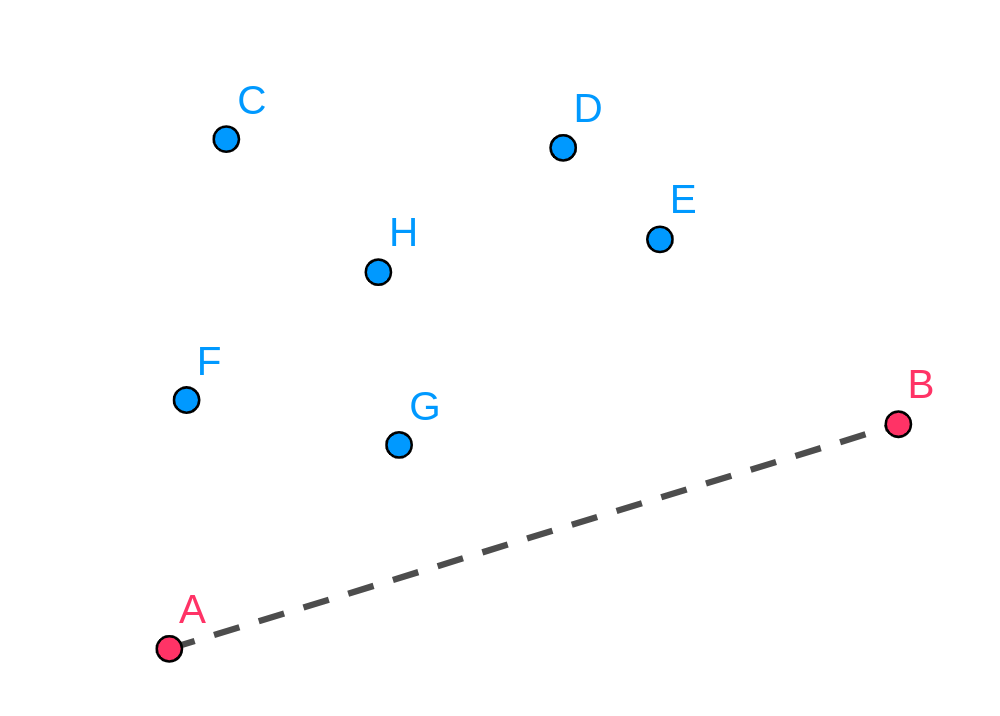
\includegraphics[width=5cm]{qh2d/geogebra-export.png}
		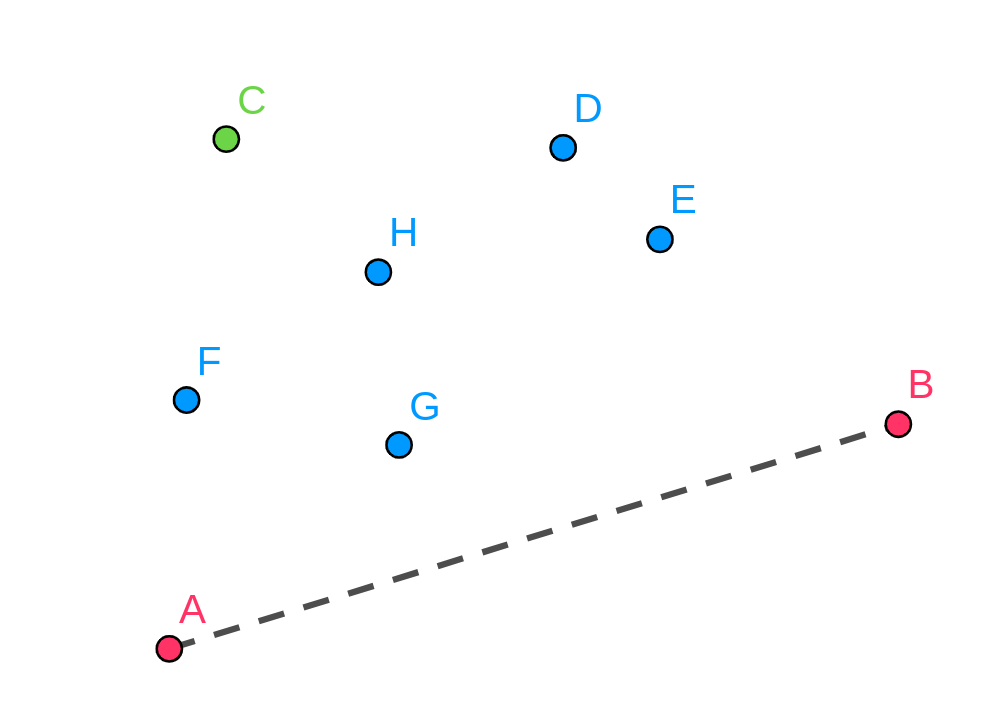
\includegraphics[width=5cm]{qh2d/geogebra-export2.png}
		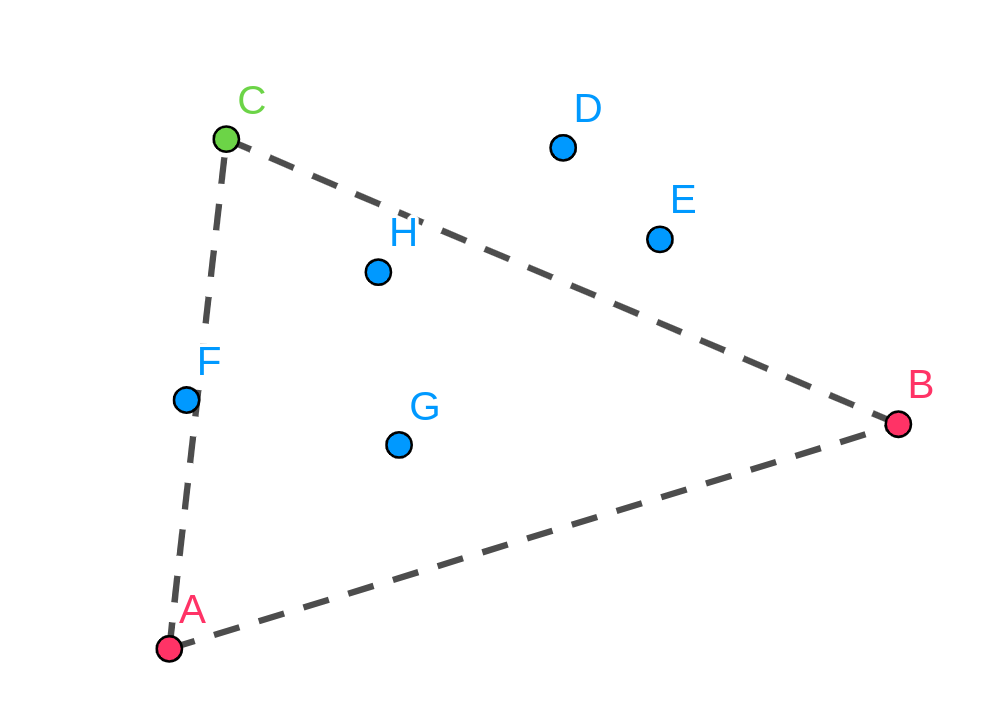
\includegraphics[width=5cm]{qh2d/geogebra-export3.png}
	\end{center}
\end{figure}

Considérons que l'on dispose des points, tels qu'illustrés ci-dessus. Supposons également que l'on sait que les points $A$ et $B$ (en rouge) appartiennent à l'enveloppe convexe (arête en pointillé). La prochaine étape de l'algorithme est alors de déterminer le point le plus extrême (c'est à dire le plus éloigné) de l'arête $AB$ : on trouve le point $C$ (en vert).

\begin{figure}[H]
	\begin{center}
		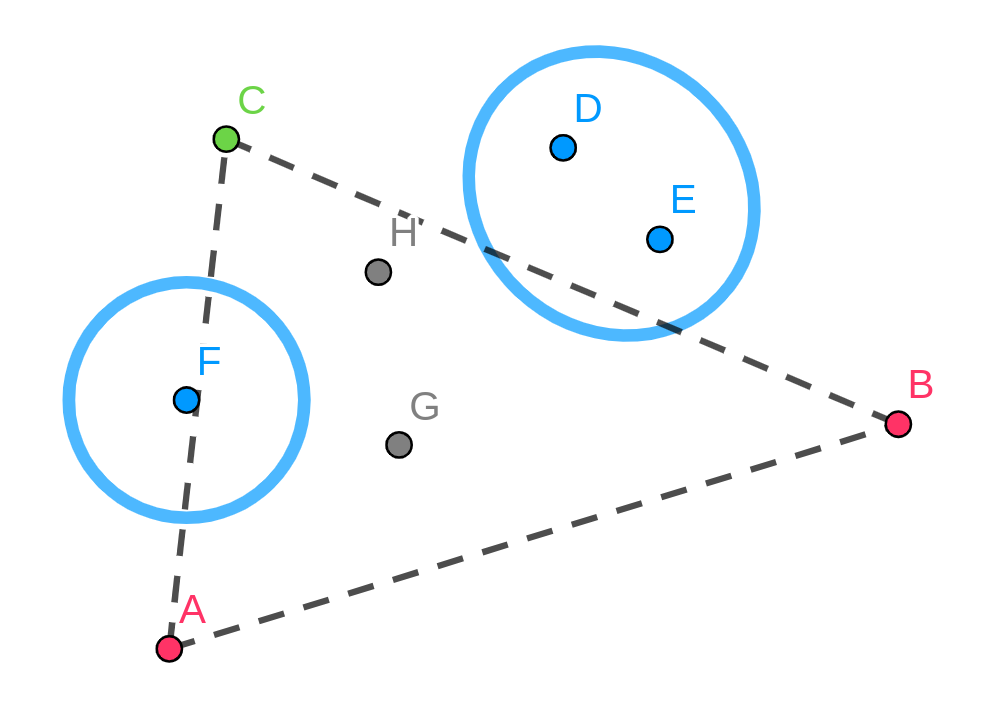
\includegraphics[width=5cm]{qh2d/geogebra-export4.png}
	\end{center}
\end{figure}

Sachant la nouvelle enveloppe obtenue, on peut procéder à la division du problème en deux sous-problèmes : pour chaque arête nouvellement créée (ici $AC$ et $CB$), on forme un sous-ensemble de points associé (entourés en bleu) en ne gardant que ceux qui sont visibles. \emph{Ici $H$ et $G$ ne sont pas visibles (les arêtes sont orientées), ni par $AC$, ni par $CB$, donc ils ne font pas partie de l'enveloppe convexe.}

On peut alors récursivement appliquer le même algorithme sur les deux sous-ensembles générés (entourés en bleu ici) par rapport à leur arête respective ($AC$ et $CB$). L'enveloppe convexe est implicitement construite par les opérations de combinaison des données de retour des sous-appels récursifs (il s'agit basiquement d'une liste ordonnée des points appartenant à l'enveloppe convexe).

\paragraph{}
La première étape de Quickhull en 2D (et donc des premiers appels récursifs) peut varier en fonction des implantations. Pour ma part j'ai choisi celle qui consiste à prendre les deux points sur un même axe ($x$ ou $y$) qui sont les plus éloignés l'un de l'autre. On obtient une arête dont chacune des extrêmités appartient à l'enveloppe convexe. Il suffit alors de lancer l'algorithme précédent en partant successivement de chacun des deux côtés de l'arête.

\subsection{Structures de données}
En termes de structures de données il n'y a besoin que de trois structures principales :
\begin{itemize}
	\item Un point constitué de deux coordonnées flottantes : $x$ et $y$.
	\item Une liste (statique) de points dont on va chercher à calculer l'enveloppe convexe.
	\item Une liste (dynamique) d'entiers non signés pour représenter aussi bien les ensembles de points (indices des points) associés à une arête, que ceux formant l'enveloppe convexe (cette liste est ordonnée dans l'ordre de voisinage des sommets des arêtes).
\end{itemize}

Du fait de la simplicité de ces structures, elles ne représentent pas une contrainte particulière pour une implantation en style fonctionnel.

\subsection{Implantation et démo visuelle}
En plus d'implanter Quickhull en 2D, j'ai développé un affichage en WebGL qui permet de visualiser et de naviguer entre les étapes de l'algorithme, sur des exemples. La visualisation est un moyen de vérifier mais aussi de mieux comprendre le fonctionnement de ce qui est implanté.

Les captures qui suivent sont celles dudit affichage, avec le code couleur suivant :
\begin{itemize}
	\item Petits points blancs : ensemble de points dont on souhaite calculer l'enveloppe convexe.
	\item Arête rouge : arête déjà parcourue qui appartient (ou qui a appartenu) à l'enveloppe convexe.
	\item Arête jaune : arête courante sur laquelle la récursion est faite ou arête nouvellement ajoutée à l'enveloppe convexe.
	\item Arête verte : arête appartenant à l'enveloppe convexe finale calculée.
\end{itemize}

\begin{figure}[H]
	\begin{center}
		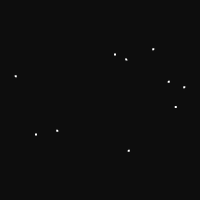
\includegraphics[width=2.5cm]{qh2d/demo2d/frame0.png}
		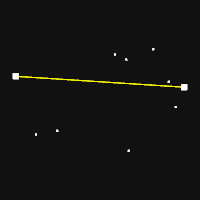
\includegraphics[width=2.5cm]{qh2d/demo2d/frame1.png}
		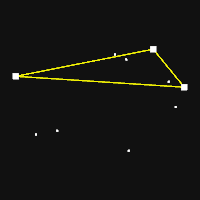
\includegraphics[width=2.5cm]{qh2d/demo2d/frame2.png}
		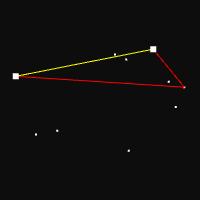
\includegraphics[width=2.5cm]{qh2d/demo2d/frame3.png}
		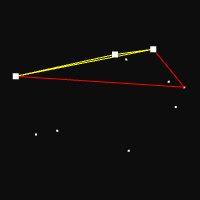
\includegraphics[width=2.5cm]{qh2d/demo2d/frame4.png}
		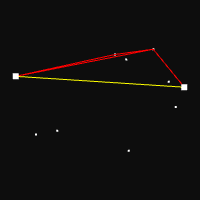
\includegraphics[width=2.5cm]{qh2d/demo2d/frame5.png}
		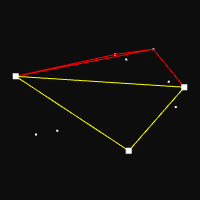
\includegraphics[width=2.5cm]{qh2d/demo2d/frame6.png}
		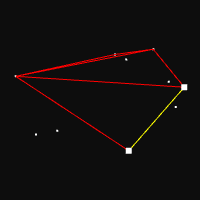
\includegraphics[width=2.5cm]{qh2d/demo2d/frame7.png}
		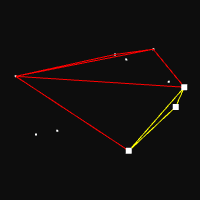
\includegraphics[width=2.5cm]{qh2d/demo2d/frame8.png}
		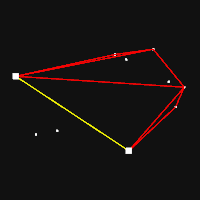
\includegraphics[width=2.5cm]{qh2d/demo2d/frame9.png}
		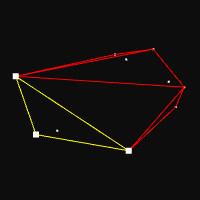
\includegraphics[width=2.5cm]{qh2d/demo2d/frame10.png}
		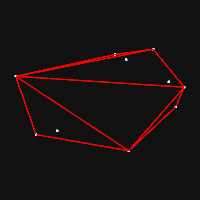
\includegraphics[width=2.5cm]{qh2d/demo2d/frame11.png}
		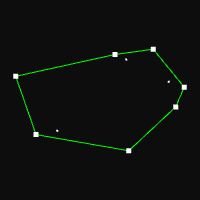
\includegraphics[width=2.5cm]{qh2d/demo2d/frame12.png}
	\end{center}
	\caption{Étapes de construction dans l'ordre chronologique de l'enveloppe convexe 2D sur un exemple simple.}
\end{figure}

\begin{figure}[H]
	\begin{center}
		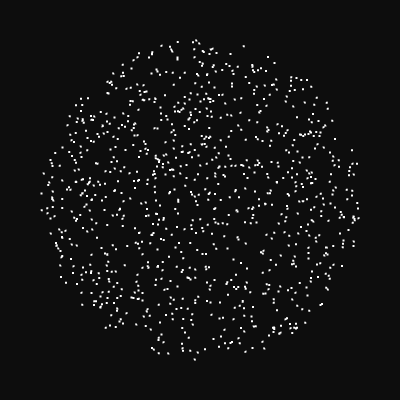
\includegraphics[width=4.5cm]{qh2d/demo2d/frame_b0.png}
		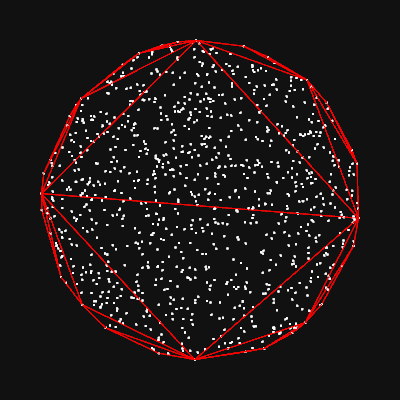
\includegraphics[width=4.5cm]{qh2d/demo2d/frame_b1.png}
		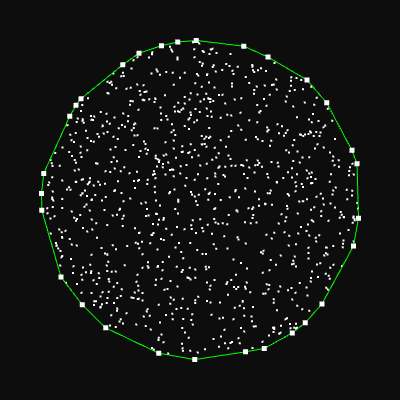
\includegraphics[width=4.5cm]{qh2d/demo2d/frame_b2.png}
	\end{center}
	\caption{Exemple avec un ensemble de points plus grand, sans toutes les étapes intermédiaires.}
\end{figure}

\pagebreak
\section{Implantation de Quickhull en 3D en JavaScript}
Implanter Quickhull restreint aux ensembles de points en 2D s'est révélé être assez simple, même en sachant la contrainte de devoir programmer en style fonctionnel. Dans cette section on s'attarde sur la version en 3D, qui représente la partie la plus importante de mon travail de recherche.

\subsection{Principe et spécificités}
Au-delà de deux dimensions, l'algorithme Quickhull est nettement plus complexe à implanter. Déjà, en trois dimensions une enveloppe convexe n'est plus une suite d'arêtes mises bout à bout, mais un maillage surfacique triangulaire. Ce qui va demander de penser à une nouvelle structure de données adaptée.

De plus, il n'est plus possible de faire un algorithme en \emph{diviser pour régner}, et pour le comprendre on va regarder un exemple similaire à celui donné pour Quickhull 2D.

\paragraph{}
\emph{Pour aider à la lisibilité des illustrations : le triangle $ABC$ est sur le plan de la grille dessinée, et des droites perpendiculaires à ce plan passent par les points $D$ à $H$.}

\begin{figure}[H]
	\begin{center}
		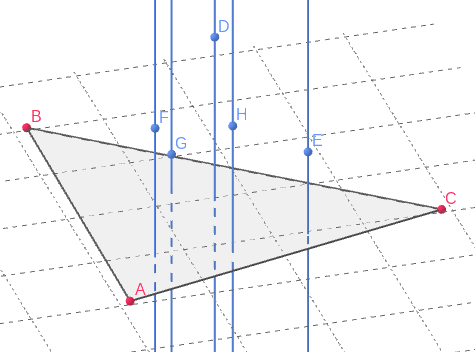
\includegraphics[width=5cm]{qh3d/geogebra-export3.png}
		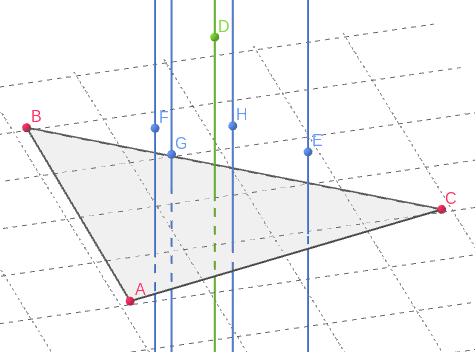
\includegraphics[width=5cm]{qh3d/geogebra-export4.png}
		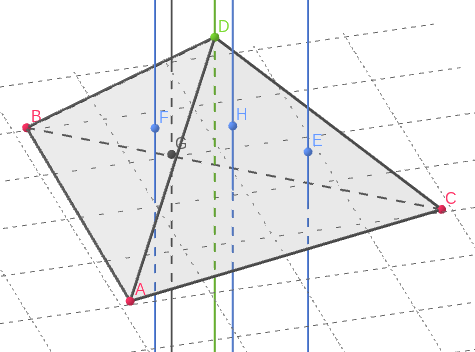
\includegraphics[width=5cm]{qh3d/geogebra-export5.png}
	\end{center}
\end{figure}

Considérons que nous disposons du triangle $ABC$ comme étant une face de l'enveloppe convexe, et des points $D$ à $H$ comme étant l'ensemble des points non traités. Comme pour Quickhull 2D, on va déterminer le point le plus extrême (c'est à dire le plus éloigné) de la face $ABC$ : on trouve le point $D$ (en vert).

La nouvelle enveloppe est alors obtenue par la construction des trois faces $ABD$, $ACD$ et $BCD$. Le prédicat de visibilité nous permet de déterminer que le point $G$ (en gris) n'appartient pas à l'enveloppe convexe, car non visible des trois faces nouvellement créées.

\paragraph{}
Tout semble bien se passer, jusqu'à l'hypothétique étape de division du problème :

\begin{figure}[H]
	\begin{center}
		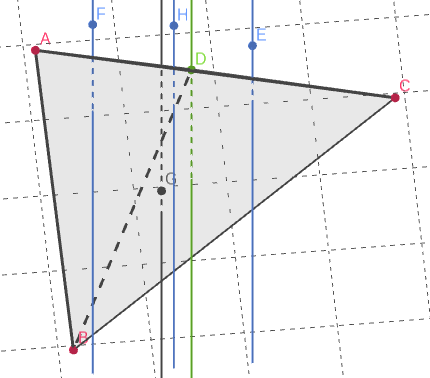
\includegraphics[width=6cm]{qh3d/geogebra-export6.png}
		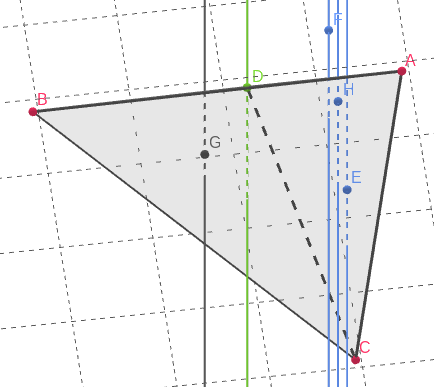
\includegraphics[width=6cm]{qh3d/geogebra-export7.png}
	\end{center}
\end{figure}

Sur ces deux vues, la caméra est orientée de telle sorte que, successivement, les faces $ACD$ puis $ABD$ nous apparaissent comme une droite. De cette manière, on met en évidence que les points $H$ et $E$ sont visibles par la face $ACD$, et non pas par la face $ABD$. Ce qui n'est pas le cas du point $F$, qui lui est visible simultanément par les deux faces.

Cette particularité nous interdit de faire l'étape de la division de \emph{diviser pour régner}, car on ne peut pas faire de subdivision en des sous-ensembles disjoints (l'un des sous-ensembles pourrait tout à fait avoir un impact sur l'autre lors du traitement). On comprend également que, contrairement à la version 2D où l'on se contentait d'agir sur une arête à la fois pour la subdiviser en de nouvelles sous-arêtes, ici on devra parfois supprimer plusieurs faces — car toutes visibles depuis un unique point extrême — pour reconstruire un certain nombre de faces supplémentaires. \emph{L'exemple donné ici est un cas particulier plutôt simple, car le point extrême $D$ ne voit qu'une seule face : le triangle $ABC$}.

\subsection{Adaptation de l'algorithme}

Puisque l'on ne peut pas faire de \emph{diviser pour régner}, l'algorithme doit être pensé différemment. Je me suis basé sur le pseudo-code donné dans \cite{10.1145/235815.235821} qui propose une généralisation pour les dimensions supérieures à 2.

\paragraph{}
La boucle principale de l'algorithme suit ces étapes :
\begin{itemize}
	\item On choisit une face parmi les faces de l'enveloppe convexe courante dont le sous-ensemble de points non-traités associé est non-vide.
	\item On prend le point le plus extrême (le plus éloigné) par rapport à ladite face depuis le sous-ensemble de points associé.
	\item On supprime \textbf{toutes} les faces visibles de l'enveloppe convexe depuis ce point.
	\item On reconstruit l'enveloppe convexe en formant des faces (triangles) entre ce point et le bord du trou laissé à l'étape précédente.
	\item On recalcule le sous-ensemble de points associé à la face courante par rapport à la nouvelle enveloppe obtenue. On devrait obtenir un nouveau sous-ensemble de points par face nouvellement ajoutée.
	\item Ré-itérer jusqu'à ce qu'il n'y ait plus de sous-ensemble non-vide associé à l'une des faces de l'enveloppe convexe.
\end{itemize}
\textbf{Note :} Un pseudo-code donné à la section \ref{pseudo-code_implantation} vient préciser l'algorithme d'une manière plus formelle.

\paragraph{}
La première étape de l'algorithme consiste (à la manière de Quickhull 2D) à trouver un solide minimal qui formera l'enveloppe convexe initiale. Celui-ci est formé de 4 faces (soient quatre points), sélectionnés d'après la méthode suivante (méthode adaptée de \cite{smith}) :
\begin{itemize}
	\item On cherche deux points les plus éloignés sur deux axes (parmi $x$, $y$ et $z$) parmi l'ensemble de points.
	\item Avec l'arête formée des deux points précédents, on cherche un troisième point le plus éloigné de ce segment.
	\item On dispose maintenant d'une face (un triangle) depuis laquelle on va chercher un quatrième point qui en est le plus éloigné.
	\item On peut dès lors construire le tétrahèdre formé par ces 4 points.
	\item On attribue (arbitrairement) à chaque face un sous-ensemble de points qui lui sont visibles.
\end{itemize}

\paragraph{}
On se rend compte que cette fois-ci il va nous falloir une structure de données pour représenter les sous-ensembles de points associés aux faces. Par la suite celle-ci sera appelée $oset$ pour \emph{outside set} (et $osubset$ pour \emph{outside subset}).

\subsection{Structures de données}
\subsubsection{Données d'entrées}
Un $vec3$ permet de modéliser aussi bien un point qu'un vecteur dans l'espace 3D. Les composantes sont données dans l'ordre usuel $x$, $y$ et $z$ (avec $x, y, z \in \mathbf{R}$).\\
Dans notre implantation, on considèrera une simple liste ordonnée des $n$ points (représentée par la variable globale $GLOBAL\_V\_LIST$) comme étant les données d'entrée du problème à résoudre.

\subsubsection{Stockage et manipulation de l'enveloppe convexe en mémoire}
La structure en liste de demi-arêtes orientées (doubly connected edge list, abrégé DCEL) est parmi les plus communes qu'il soit dès lors que l'on souhaite modéliser un maillage topologique.\\
Ici on implante une version restreinte de cette dernière, puisqu'elle permet de créer maillages triangulaires uniquement — ce qui correspond à notre besoin.

\paragraph{Demi-arête}
Une $he$ (abrévation de halfedge, ou demi-arête) est une structure de données disposant d'informations sur elle-même et son voisinage topologique. Les champs et leur sémantique associée sont les suivants :
\begin{itemize}
	\item $index \in \mathbf{Z}$, un identifiant unique pour la demi-arête, avec :
	      \[
		      \left\{
		      \begin{array}{ll}
			      index = -1   & \mbox{est une demi-arête nulle} \\
			      index \geq 0 & \mbox{sinon}
		      \end{array}
		      \right.
	      \]
	\item $opposite \in \mathbf{Z}$, l'identifiant de la demi-arête opposée, avec :
	      \[
		      \left\{
		      \begin{array}{ll}
			      opposite = -1   & \text{est une demi-arête du bord} \\
			      opposite \geq 0 & \text{sinon}
		      \end{array}
		      \right.
	      \]
	\item $vertex \in \mathbf{N}$, l'indice du sommet incident dont elle est issue.
\end{itemize}

\paragraph{Maillage triangulaire}
Une $dcel$ permet la modélisation d'un maillage topologique triangulaire. Elle dispose des attributs suivants :
\begin{itemize}
	\item $he\_list$, une liste de $he$.
	\item $available\_he\_index \in \mathbf{N}$, le prochain indice non attribué à une $he$ de la liste.
\end{itemize}

\paragraph*{Exemple simple en 2D}
Considérons le maillage de la Figure~\ref{maillage_simple}. Une structure $dcel$ associée valide serait alors telle que celle présentée Figure~\ref{maillage_simple_struct_associee}.

\begin{figure}[H]
	\[\begin{aligned}[c]
			\entrymodifiers={+[o][F]}
			\renewcommand{\labelstyle}{\textstyle}
			\xymatrix@=4em @L=.25ex{
			{}
			\ar @^{-} [d]
			\ar @^{-} [dr]
			 & {}
			\ar @^{-} [l]
			\\ {}
			\ar @^{-} [r]
			 & {}
			\ar @^{-} [u]
			}
		\end{aligned}\rightarrow\begin{aligned}[c]
			\xymatrix@=4em @L=.25ex{
			{\color{red}0}
			\ar @<.25ex> @^{->} [d] |{\color{blue}0}
			\ar @<.25ex> @^{->} [dr] ^{\color{blue}4}
			 & {\color{red}1}
			\ar @<.25ex> @^{->} [l] |{\color{blue}3}
			\\ {\color{red}2}
			\ar @<.25ex> @^{->} [r] |{\color{blue}1}
			 & {\color{red}3}
			\ar @<.25ex> @^{->} [ul] ^{\color{blue}2}
			\ar @<.25ex> @^{->} [u] |{\color{blue}5}
			}
		\end{aligned}\]
	\caption{Un maillage simple et un indiçage correspondant.}
	\label{maillage_simple}
\end{figure}

\begin{figure}[H]
	\[
		\begin{aligned}[c]
			\begin{array}{l}
				\begin{tabular}{|c|c|c|c|}
					\hline
					index         & opposite      & vertex       \\
					\hline
					\color{blue}0 & -1            & \color{red}0 \\
					\hline
					\color{blue}1 & -1            & \color{red}2 \\
					\hline
					\color{blue}2 & \color{blue}4 & \color{red}3 \\
					\hline
					\color{blue}3 & -1            & \color{red}1 \\
					\hline
					\color{blue}4 & \color{blue}2 & \color{red}0 \\
					\hline
					\color{blue}5 & -1            & \color{red}3 \\
					\hline
				\end{tabular} \\\\
				available\_he\_index\textbf{ : }6
			\end{array}
		\end{aligned}
		\begin{aligned}[c]
			\begin{tabular}{|c|c|}
				\hline
				Indice       & Coordonnées \\
				\hline
				\color{red}0 & (0,0)       \\
				\hline
				\color{red}1 & (1,0)       \\
				\hline
				\color{red}2 & (1,1)       \\
				\hline
				\color{red}3 & (0,1)       \\
				\hline
			\end{tabular}
		\end{aligned}
	\]
	\caption{Structure $dcel$ à gauche et la table des sommets à droite.}
	\label{maillage_simple_struct_associee}
\end{figure}

\textbf{Note :} $avaiable\_he\_index$ est l'indice pour la prochaine demi-arête qui sera ajoutée à la $dcel$. On pourrait s'en passer et utiliser à la place l'indice de la dernière $he$ ajoutée à la $dcel$ pour calculer le prochain indice.\\

\textbf{Note :} Il n'y a que deux opérations principales de modification d'une $dcel$ : l'ajout d'une face, et le retrait d'une face. L'ajout d'une face correspond à l'ajout de trois demi-arêtes, et le retrait d'une face correspond à la suppression de trois demi-arêtes.

\subsubsection{Stockage et manipulation de l'ensemble de points extérieurs associés aux faces}
\paragraph*{Sous-ensemble de points extérieurs — $osubset$}
Un sous-ensemble de points extérieurs (outside subset) est une structure de données à deux champs :
\begin{itemize}
	\item $face\_index \in \mathbf{N}$, l'identifiant unique d'une face.
	\item $list \in \mathbf{N}$, l'ensemble des points extérieurs à la face $face\_index$, représentés par leur indice dans $GLOBAL\_V\_LIST$.
\end{itemize}

\paragraph*{Ensemble de points extérieurs — $oset$}
L'ensemble de points extérieurs (outside set) n'est rien d'autre qu'une liste de couples d'$osubset$ et d'indice de face associée.

\subsection{Propriétés et spécifications supplémentaires des structures de données}
Avec toutes les informations dont on dispose sur les structures de données, on peut alors en déduire des propriétés et des spécifications plus détaillées.\\

Soit $P \subset \mathbf{R^3} $, l'ensemble $n$ des points tridimensionnels donnés en entrée de Quickhull.\\
Soit $P_{indices}$ = $\{0,1,\ldots,n - 1\}$, l'ensemble des $n$ indices associés aux $n$ points de $P$.\\
Soit $O$ un $oset$, l'ensemble des couples $\langle f, O_{subset} \rangle$ de faces et de points extérieurs associés.\\
Soit $E$ une $dcel$, l'ensemble des $m$ demi-arêtes de l'enveloppe.\\

Alors à tout moment, les propriétés suivantes sur les structures de données sont censées être vérifiées pour être considérées comme étant valides :
\begin{itemize}
	\item La taille de $E$ (son nombre de demi-arêtes) est un multiple de 3.
	\item Pour toute demi-arête $he \in E$ :
	      \[
		      0 \leq he.index < m
	      \]
	      \[
		      -1 \leq he.opposite < m
	      \]
	      \[
		      he.vertex \in P_{indices}
	      \]
	\item Les sous-ensembles de points sont disjoints :
	      \[
		      \emptyset = \bigcap_{\langle f, O_{subset} \rangle \in O}^{} { O_{subset}}
	      \]
	\item L'union des sous-ensembles de points est inclus dans l'ensemble $P_{indices}$ :
	      \[
		      P_{indices} \supseteq \bigcup_{\langle f, O_{subset} \rangle \in O}^{} O_{subset}
	      \]
	\item Pour tout couple $\langle face_{indice}, O_{subset} \rangle \in O$:
	      \[
		      0 \leq face_{indice} < \lfloor m / 3 \rfloor
	      \]
	      \textbf{Note :} Cette dernière propriété implique que la structure $oset$ doit être maintenue à jour après chaque modification de la structure $dcel$. C'est illustré dans la section \ref{pseudo-code_implantation}, algo. \ref{algo_Quickhull3DRec}, ligne \ref{maj_oset_instr}.
\end{itemize}

\pagebreak
\subsection{Pseudo-code}\label{pseudo-code_implantation}

\subsubsection{Fonctions principales}

\begin{algorithm}[H]
	\caption{Quickhull3D}
	\begin{algorithmic}[1]
		\Require $P$ une liste de points tridimensionnels dont on veut calculer l'enveloppe convexe 3D
		\Function{Quickhull3D}{$P$}
		\State $P_{indices} \leftarrow$ \Call{listeOrdonneeEntiers}{$P$}
		\State $\langle E_{initiale}, O_{initial} \rangle \leftarrow$ \Call{tetrahedreInitial}{$P_{indices}$}
		\State \Return \Call{Quickhull3DRec}{$P$, $E_{initiale}$, $O_{initial}$}
		\EndFunction
	\end{algorithmic}
\end{algorithm}

L'algorithme qui suit, bien que récursif, est équivalent à une boucle \texttt{while}.
\begin{algorithm}[H]
	\caption{Quickhull3DRec}
	\label{algo_Quickhull3DRec}
	\begin{algorithmic}[1]
		\Require $P$ la liste des points 3D (reste inchangée lors de l'exécution)
		\Require $E$ une $dcel$ (enveloppe)
		\Require $O$ un $oset$ (ensemble des sous-ensembles de points extérieurs associés aux faces de $E$)
		\Function{Quickhull3DRec}{$P$, $E$, $O$}
		\If{$O = \emptyset$}
		\State \Return $E$
		\Else
		\State $\langle f_{sel}, O_{sel} \rangle \leftarrow$ \Call{premierOsubset}{$O$} \Comment{$\langle f_{sel}, O_{sel} \rangle \in O$} \label{heuristique2}
		\State $p_{sel} \leftarrow$ \Call{lePlusEloigne}{$P$, $f_{sel}$, $O_{sel}$} \Comment{$p_{sel} \in O_{sel}$} \label{heuristique1}
		\State Retirer $p_{sel}$ du sous-ensemble associé à la face $f_{sel}$ de $O$
		\State $\langle E, F_{suppr} \rangle \leftarrow$ \Call{supprimerFacesVisibles}{$P$, $E$, $f_{sel}$, $p_{sel}$}
		\State $\langle E, F_{creees} \rangle \leftarrow$ \Call{reconstruireFaces}{$E$, $p_{sel}$}
		\State $O \leftarrow$ \Call{mettreAjourOset}{$P$, $E$, $O$, $F_{suppr}$, $F_{creees}$}\label{maj_oset_instr}
		\State \Return \Call{Quickhull3DRec}{$P$, $E$, $O$}
		\EndIf
		\EndFunction
	\end{algorithmic}
\end{algorithm}


\paragraph{Invariant à noter ici} Soient $E_i$ et $E_{i + 1}$ des $dcel$, $O_i$ et $O_{i + 1}$ les $oset$, respectivement au début de la récursion $i$ et de la sous-récursion $i + 1$ de l'algorithme, on peut déduire l'invariant suivant :
\[
	\left(\bigcup_{\langle f, O_{subset} \rangle \in O_{i + 1}}^{} O_{subset} \right) \subset \left(\bigcup_{\langle f, O_{subset} \rangle \in O_i}^{} O_{subset} \right)
\]
En effet, à chaque récursion (ou  itération) on est certain de supprimer au moins un point dans l'$oset$ : le point extrême sélectionné. Cet invariant assure la terminaison de l'algorithme.\\

\textbf{Note :} L'appel à la fonction \texttt{lePlusEloigne} a un coût en $O(n)$, $n$ étant la taille du sous-ensemble $O_{sel}$, ce qui est acceptable.

\subsubsection{Supression des faces visibles}
Cet algorithme supprime les faces de l'enveloppe $E$, visibles depuis le point $p_{sel}$. En apparence plutôt complexe, son principe reste assez simple. Il part de la face $f$, la supprime (ligne \ref{suppr_face}, algo. \ref{algo_supprimerFacesVisibles}), puis, récursivement, explore et supprime ses faces voisines. Les conditions d'arrêt sont que : la face explorée ne soit plus visible depuis $p_{sel}$ (ligne \ref{visible_cond}, algo. \ref{algo_supprimerFacesVisiblesRec}), ou que la face explorée ait déjà été supprimée (ligne \ref{bordure_cond}, algo. \ref{algo_supprimerFacesVisiblesRec}), auquel cas on est sur une arête de bordure.

Une illustration donnée à la section \ref{demo_visuelle_3d_js}, figure \ref{demo_visuelle_3d_js_fig_a}, correspond à cet algorithme.

\begin{algorithm}[H]
	\caption{supprimerFacesVisibles}
	\label{algo_supprimerFacesVisibles}
	\begin{algorithmic}[1]
		\Require $P$ la liste des points 3D (reste inchangée lors de l'exécution)
		\Require $E$ une $dcel$
		\Require $f$ l'indice de la face sélectionnée
		\Require $p$ l'indice du point sélectionné
		\Function{supprimerFacesVisibles}{$P$, $E$, $f$, $p$}
		\State $E \leftarrow$ \Call{supprimerFace}{$E$, $f$} \label{suppr_face}
		\State $F_{suppr} \leftarrow \{ f \}$
		\For{chaque arête $he$ de la face $f$}
		\State $\langle E, F_{suppr} \rangle \leftarrow$ \Call{supprimerFacesVisiblesRec}{$P$, $\langle E, F_{suppr} \rangle$, $he$, $p$}
		\EndFor
		\State \Return $\langle E, F_{suppr} \rangle$
		\EndFunction
	\end{algorithmic}
\end{algorithm}

\begin{algorithm}[H]
	\caption{supprimerFacesVisiblesRec}
	\label{algo_supprimerFacesVisiblesRec}
	\begin{algorithmic}[1]
		\Require $P$ la liste des points 3D (reste inchangée lors de l'exécution)
		\Require $E$ une $dcel$
		\Require $F_{suppr}$ une liste d'indices des faces supprimées
		\Require $he_{oppo}$ la demi-arête d'où l'on vient, opposée à la demi-arête où l'on va
		\Require $p$ l'indice du point sélectionné (constant)
		\Function{supprimerFacesVisiblesRec}{$P$, $\langle E, F_{suppr} \rangle$, $he_{oppo}$, $p$}
		\If{ !\Call{estEnBordure}{$he_{oppo}$}} \label{bordure_cond}
		\State $he \leftarrow$ \Call{demiAreteOpposee}{$he_{oppo}$}
		\State $f \leftarrow$ \Call{indiceDeFace}{$he$}
		\If{\Call{estVisible}{$P$, $E$, $p$, $f$}} \label{visible_cond}
		\State $E \leftarrow$ \Call{supprimerFace}{$E$, $f$}
		\State $F_{suppr} \leftarrow F_{suppr} \cup \{ f \}$
		\State $\langle E, F_{suppr} \rangle \leftarrow \Call{supprimerFacesVisiblesRec}{$P$, \langle E, F_{suppr} \rangle, \Call{demiAretePrec}{he}, p}$
		\State $\langle E, F_{suppr} \rangle \leftarrow \Call{supprimerFacesVisiblesRec}{$P$, \langle E, F_{suppr} \rangle, \Call{demiAreteSuiv}{he}, p}$
		\EndIf
		\EndIf
		\State \Return $\langle E, F_{suppr} \rangle$
		\EndFunction
	\end{algorithmic}
\end{algorithm}

\subsubsection{Reconstruction des faces}
L'algorithme précédent a conduit à la supression de faces dans l'enveloppe $E$. La reconstruction consiste à construire un triangle entre chaques demi-arêtes de la bordure de $E$ et le point extrême $p_{sel}$. La bordure est obtenue en un temps linéaire, par parcours et récupération des demi-arêtes de $E$ qui sont des demi-arêtes de bordure ($he.opposite == -1$).

Une illustration donnée à la section \ref{demo_visuelle_3d_js}, figure \ref{demo_visuelle_3d_js_fig_a}, correspond à cet algorithme.
\begin{algorithm}[H]
	\caption{reconstruireFaces}
	\begin{algorithmic}[1]
		\Require $E$ une $dcel$, $p$ l'indice du point sélectionné
		\Function{reconstruireFaces}{$E$, $p_{sel}$}
		\State $HE_{bord} \leftarrow$ \Call{demiAretesDuBord}{$E$} \Comment {$HE_{bord} \subseteq E$}
		\State $F_{creees} \leftarrow \emptyset$
		\For{chaque demi-arête $he$ de $HE_{bord}$}
		\State $E \leftarrow$ \Call{ajouterFace}{$E$, $he$, $p$}
		\State $F_{creees} \leftarrow F_{creees} \cup \{ \Call{indiceDeFace}{\Call{demiAreteOppos}{he}} \}$
		\EndFor
		\State \Return $\langle E, F_{creees} \rangle$
		\EndFunction
	\end{algorithmic}
\end{algorithm}

\subsubsection{Mise à jour de l'ensemble de points extérieurs}
L'appel à cette méthode se fait dans un contexte où l'on a déjà supprimé puis reconstruit des faces. Notre $oset$ contient encore les faces qui ont été supprimées avec leurs points associés, et pas celles qui ont été créées.

On supprime les sous-ensembles de points associés à des faces supprimées ligne \ref{suppr_faces_oset}, et on garde dans une liste à part les points devenus orphelins, ligne \ref{rapp_points_oset}. Dans la boucle, ligne \ref{faces_creees_oset}, on ajoute à l'$oset$, des sous-ensembles extérieurs vides, associés aux faces nouvellement créées. Lignes \ref{assoc_oset} à \ref{assoc_oset2}, pour chaque point orphelin, on recherche parmi les nouvelles faces une pour laquelle il est visible. Si tel est le cas, ce point est ajouté au sous-ensemble correspondant de l'$oset$, sinon cela signifie qu'il a été capturé dans le volume de la nouvelle enveloppe convexe (auquel cas il est oublié). La ligne \ref{suppr_vide_oset} supprime les sous-ensembles vides de l'$oset$ (ça n'est pas obligatoire en fonction de l'implantation).
\begin{algorithm}[H]
	\caption{mettreAjourOset}
	\begin{algorithmic}[1]
		\Require $P$ la liste des points 3D (reste inchangée lors de l'exécution)
		\Require $E$ une $dcel$
		\Require $O$ un $oset$
		\Require $F_{suppr}$ la liste d'indices des faces qui ont été supprimées
		\Require $F_{creees}$ la liste d'indices des faces qui ont été créées
		\Function{mettreAjourOset}{$P$, $E$, $O$, $F_{suppr}$, $F_{creees}$}
		\State $V_{atraiter} \leftarrow \emptyset$
		\For{chaque couple $\langle f, O_{subset} \rangle$ de $O$}
		\If{$f \in F_{suppr}$}
		\State $V_{atraiter} \leftarrow V_{atraiter} \cup O_{subset}$ \label{rapp_points_oset}
		\State $O \leftarrow O \setminus \{\langle f, O_{subset} \rangle\}$ \label{suppr_faces_oset}
		\EndIf
		\EndFor
		\For{chaque face $f$ de $F_{creees}$} \label{faces_creees_oset}
		\State $O \leftarrow O \cup \{ \langle f, \emptyset \rangle \}$
		\EndFor
		\For{chaque point $v$ de $V_{atraiter}$} \label{assoc_oset}
		\For{chaque face $f$ de $F_{creees}$}
		\If{ \Call{estVisible}{$P$, $E$, $v$, $f$} }
		\State Ajouter $v$ dans le sous-ensemble de $f$ dans $O$
		\State \textbf{Break} \Comment{$v$ est déjà assigné à $f$, donc on peut passer au point suivant}
		\EndIf
		\EndFor
		\EndFor \label{assoc_oset2}
		\State $O \leftarrow$ \Call{supprimerSousEnsemblesVides}{$O$} \label{suppr_vide_oset}
		\State \Return $O$
		\EndFunction
	\end{algorithmic}
\end{algorithm}

\pagebreak
\subsection{Évaluation des performances}
Lors d'une itération dans l'algorithme de calcul d'enveloppe convexe 3D, deux instructions successives amènent à devoir choisir un élément parmi un ensemble — sachant que tous conduisent à la terminaison du programme et à la construction d'une enveloppe convexe valide. Dès lors l'utilisation d'heuristiques est envisageable, et cette partie porte sur la comparaison des performances en temps de calcul en fonction des méthodes employées.

Les tests ont été conduits en moyennant le temps de calcul pour 50 échantillons de points générés aléatoirement (répartition spatiale aléatoire et uniforme).

\paragraph{Heuristique sur le choix du point}
Ici on s'intéresse à la sélection du point parmi ceux du sous-ensemble choisit. Correspond à la ligne \ref{heuristique1} de l'algorithme \ref{algo_Quickhull3DRec}, section \ref{pseudo-code_implantation}.
\begin{figure}[H]
	\begin{center}
		\begin{tikzpicture}[scale=0.8]
			\begin{axis}[
					title = {},
					xlabel = {Nombre de points en entrée},
					ylabel = {Temps de calcul (ms)},
					legend entries={Point le plus éloigné,Premier point de la liste},
					legend style={at={(0,1)},anchor=north west}
				]
				\addplot+[blue] table {medias/normal.dat};
				\addplot table {medias/not_extreme_point.dat};
			\end{axis}
		\end{tikzpicture}
	\end{center}
	\caption{La courbe bleue montre ici que la stratégie consistant à prendre le point le plus éloigné du plan courant offre de meilleures performances en temps que celle où l'on prend naïvement le premier point de la liste (courbe rouge).}
\end{figure}

\paragraph{Heuristique sur le choix du sous-ensemble} Ici on s'intéresse à la sélection du prochain sous-ensemble de points non-vide (et donc implicitement d'une face du polygone convexe en cours de construction). Correspond à la ligne \ref{heuristique2} de l'algorithme \ref{algo_Quickhull3DRec}, section \ref{pseudo-code_implantation}.
\begin{figure}[H]
	\begin{center}
		\begin{tikzpicture}[scale=0.8]
			\begin{axis}[
					title = {},
					xlabel = {Nombre de points en entrée},
					ylabel = {Temps de calcul (ms)},
					legend entries={Premier sous-ensemble,Plus petit sous-ensemble,Plus grand sous-ensemble},
					legend style={at={(0,1)},anchor=north west},
				]
				\addplot+[blue] table {medias/normal.dat};
				\addplot table {medias/smallest_osubset.dat};
				\addplot table {medias/largest_osubset.dat};
			\end{axis}
		\end{tikzpicture}
	\end{center}
	\caption{
		De manière prévisible choisir le plus petit sous-ensemble à chaque itération nuit aux performances de l'algorithme (courbe rouge). En effet en ne prenant à chaque fois que un plus petit sous-ensemble de $n$ points (avec $n > 0$), on se restreint alors à retirer de l'ensemble total $n$ points au mieux à cette itération.\\
		Il est intéressant de noter ici que prendre le plus grand sous-ensemble (courbe brune) est plus performant que de choisir le premier de la liste (courbe bleue), mais le gain n'est pas aussi significatif que ce qu'on a montré juste avant.
	}
\end{figure}

\subsection{Démo visuelle}\label{demo_visuelle_3d_js}
De la même manière que pour la version 2D, j'ai développé un affichage de l'algorithme de calcul d'enveloppe convexe 3D avec WebGL. Celui-ci s'est avéré absolument indispensable pour débugger le code tout au long du développement. Au final il permet également de visualiser, étape par étape, la construction des différentes faces de l'enveloppe convexe.

\begin{figure}[H]
	\begin{center}
		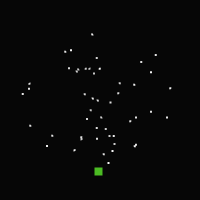
\includegraphics[width=2.65cm]{qh3d/demo3d/init_6.png}
		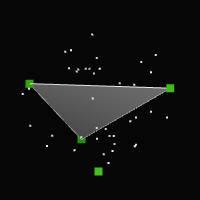
\includegraphics[width=2.65cm]{qh3d/demo3d/init_5.png}
		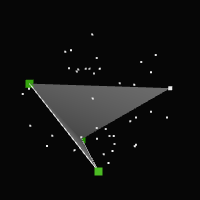
\includegraphics[width=2.65cm]{qh3d/demo3d/init_4.png}
		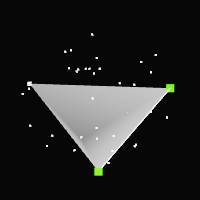
\includegraphics[width=2.65cm]{qh3d/demo3d/init_3.png}
		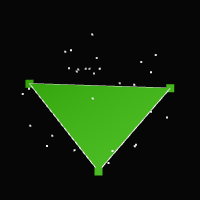
\includegraphics[width=2.65cm]{qh3d/demo3d/init_2.png}
		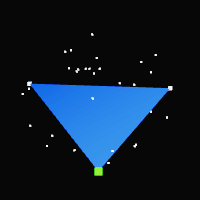
\includegraphics[width=2.65cm]{qh3d/demo3d/init_1.png}
	\end{center}
	\caption{Exemple d'étapes, dans l'ordre chronologique, de la construction de l'enveloppe initiale (tétrahèdre) sur un ensemble de points 3D, face après face.}
	\label{fig:env_initiale}
\end{figure}

\begin{figure}[H]
	\begin{center}
		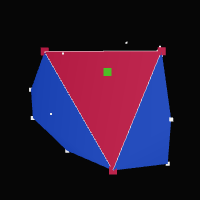
\includegraphics[width=2.65cm]{qh3d/demo3d/add_rem_10.png}
		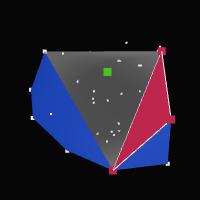
\includegraphics[width=2.65cm]{qh3d/demo3d/add_rem_9.png}
		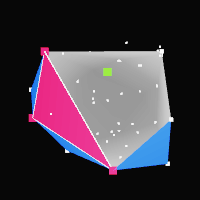
\includegraphics[width=2.65cm]{qh3d/demo3d/add_rem_8.png}
		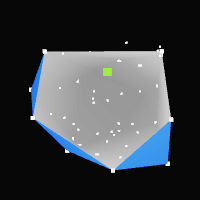
\includegraphics[width=2.65cm]{qh3d/demo3d/add_rem_7.png}
		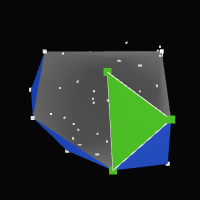
\includegraphics[width=2.65cm]{qh3d/demo3d/add_rem_6.png}
		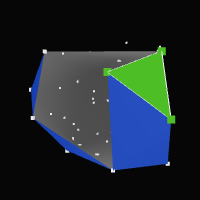
\includegraphics[width=2.65cm]{qh3d/demo3d/add_rem_5.png}
		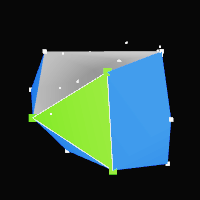
\includegraphics[width=2.65cm]{qh3d/demo3d/add_rem_4.png}
		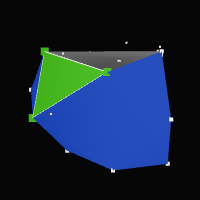
\includegraphics[width=2.65cm]{qh3d/demo3d/add_rem_3.png}
		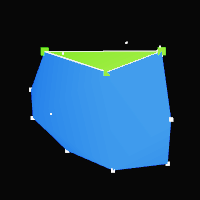
\includegraphics[width=2.65cm]{qh3d/demo3d/add_rem_2.png}
		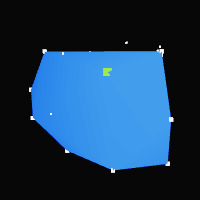
\includegraphics[width=2.65cm]{qh3d/demo3d/add_rem_1.png}
	\end{center}
	\caption{Exemple d'étapes, dans l'ordre chronologique, de la suppression des faces visibles (en rouge) depuis un point extrême sélectionné (en vert), puis de la reconstructions de nouvelles faces (en vert). Ces dernières sont obtenues en construisant les triangles entre les arêtes du bord engendré, et le point extrême sélectionné.}
	\label{demo_visuelle_3d_js_fig_a}
\end{figure}

\begin{figure}[H]
	\begin{center}
		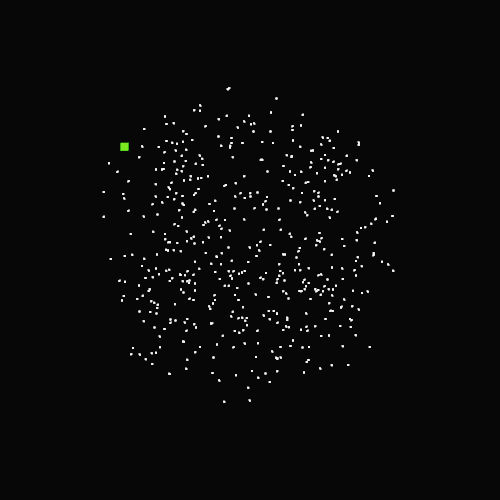
\includegraphics[width=4cm]{qh3d/demo3d/main_0.png}
		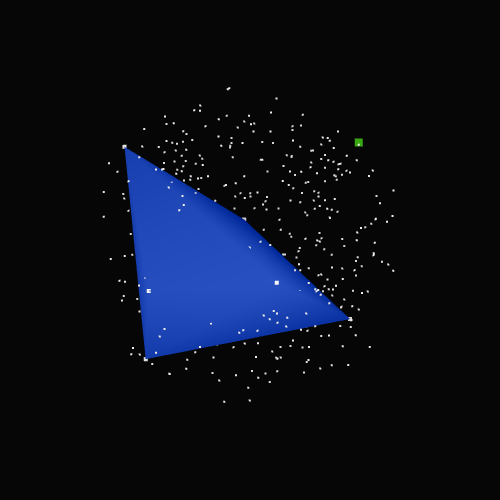
\includegraphics[width=4cm]{qh3d/demo3d/main_1.png}
		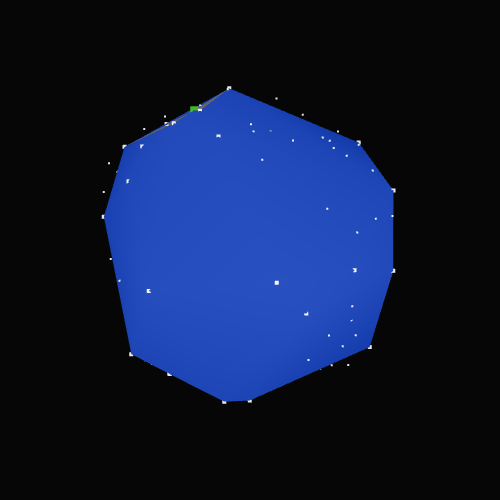
\includegraphics[width=4cm]{qh3d/demo3d/main_2.png}
		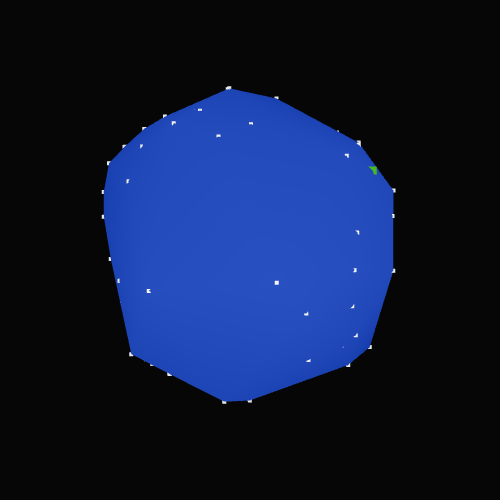
\includegraphics[width=4cm]{qh3d/demo3d/main_3.png}
	\end{center}
	\caption{Dernier exemple sur un grand ensemble de points, engendrant un nombre de faces plus élevé.}
\end{figure}

\pagebreak
\section{Implantation d'une étape de Quickhull 3D en Coq et extraction en Haskell}
Maintenant que nous avons une implantation de Quickhull 3D qui fonctionne dans un style de programmation fonctionnel, il serait intéressant d'explorer ce qu'il est possible de faire avec Coq. Pour rappel, l'idée à terme serait d'utiliser ce dernier pour prouver formellement que notre implantation de Quickhull 3D est correcte.

\subsection{Variations par rapport à l'implantation JavaScript}
Pour cette ré-implantation en Coq, je n'ai pas ré-écrit tout l'algorithme de Quickhull 3D, ni toutes ses structures de données. Le temps qu'il me restait m'aurait été bien insuffisant pour cela. L'idée c'est plutôt d'avoir une preuve de concept, et donc j'ai décidé de n'implémenter que la première partie de l'algorithme qui consiste à \textbf{calculer une enveloppe initiale} (des illustrations sont données dans les  figures \ref{fig:env_initiale} et \ref{fig:env_initiale_haskell}).

Ainsi ce que j'ai implanté sont les $vec3$ (pour représenter les points en trois dimensions), des opérations arithmétiques sur ces mêmes $vec3$, des opérations sur les listes, les $he$ et les $dcel$ avec leurs méthodes (à l'exception de l'opération de suppression de face).

\paragraph{Des détails d'implantation ont été revus par rapport à la version en JavaScript}
L'exemple le plus parlant est celui d'avoir utilisé la valeur $-1$ à chaque fois qu'il y a un indice qui peut être non-défini. En Coq (et en programmation fonctionnelle de manière générale), on peut faire mieux que cela en utilisant des monades. Les monades apportent une réelle sémantique, qui est explicite — une valeur peut-être non-définie —, contrairement au fait de choisir une valeur constante arbitraire, qui elle serait spécifique à l'implantation.

J'ai étendu l'utilisation de monades partout où cela me paraissait pertinent. Par exemple, pour les opérations d'accès par indice dans une liste. L'intérêt est aussi d'avoir des garde-fous à plusieurs endroits du programme.

\subsection{Extraction du code Coq}
Dans l'introduction, nous avons vu que Coq n'est pas fait pour exporter ou importer des fichiers, dès lors qu'il ne s'agit pas de fichiers Coq compilés. Il est aussi très limité en termes de capacités d'exécution de code.

Cependant, l'un de ses modules permet de faire ce que l'on appelle de \textbf{l'extraction de code}. Cette opération consiste à transformer du code source écrit en Coq en un code source écrit dans un autre langage fonctionnel, au choix. Ce que l'on voudrait donc c'est de pouvoir compiler ce code extrait, pour pouvoir ensuite l'exécuter et se convaincre visuellement de son fonctionnement.

\subsubsection{Choix du langage d'extraction}
Les langages d'extraction supportés par Coq sont au nombre de quatre. À savoir : OCaml, Haskell, Scheme et JSON (qui n'est pas un langage de programmation, mais de stockage de données). Vient alors la question de choisir le langage d'extraction qui sera utilisé.

\subparagraph*{JSON}
Ma première idée fut de choisir le JSON. En effet, je n'ai aucune connaissance des autres langages disponibles, et j'ai d'abord estimé qu'il serait plus long pour moi de me former à l'un de ceux-ci. De plus, le JSON est extrêmement simple à comprendre et à utiliser, il le serait d'autant plus lorsqu'il s'agira de le raccorder à ce que j'avais déjà développé en JavaScript.
\begin{figure}[H]
	\begin{center}
		\tikzstyle{myblock} = [rectangle, draw]
		\begin{tikzpicture}
			\node[myblock] (I1) {Coq};
			\node[myblock, right=of I1, xshift=2cm] (I2) {JSON};
			\node[myblock, right=of I2, xshift=2cm] (I3) {JavaScript};
			\draw[->] (I1)--node[above] {Extraction}(I2);
			\draw[->] (I2)--node[above] {?}(I3);
		\end{tikzpicture}
	\end{center}
\end{figure}
Seulement voilà, le JSON est un format de stockage de données uniquement, et donc l'agencement à l'intérieur d'un fichier est purement arbitraire. Hors, l'extraction de Coq vers ce format n'est absolument pas documentée. Il n'y a même aucune assurance pour que le code extrait soit correct.

Faire la rétro-ingénierie des fichiers extraits depuis Coq aurait été d'une part difficile, mais en plus excessivement long à réaliser, sans aucune garantie de succès. Je n'ai donc pas maintenu ce choix.

\subparagraph{OCaml}\label{OCaml_to_js}
OCaml était ma seconde option. Bien que je ne connaisse pas ce langage, j'ai découvert l'existence d'un compilateur appelé Js\_of\_ocaml, qui permet de compiler du bytecode OCaml vers du JavaScript.
\begin{figure}[H]
	\begin{center}
		\tikzstyle{myblock} = [rectangle, draw]
		\begin{tikzpicture}
			\node[myblock] (I1) {Coq};
			\node[myblock, right=of I1, xshift=2cm] (I2) {OCaml};
			\node[myblock, right=of I2, xshift=2cm] (I3) {Bytecode OCaml};
			\node[myblock, right=of I3, xshift=2cm] (I4) {JavaScript};
			\draw[->] (I1)--node[above] {Extraction}(I2);
			\draw[->] (I2)--node[above] {Compilation}(I3);
			\draw[->] (I3)--node[above] {Js\_of\_ocaml}(I4);
		\end{tikzpicture}
	\end{center}
\end{figure}
Sur le papier c'était clairement une bonne solution puisqu'elle aurait permis l'utilisation de ce que j'avais déjà fait auparavant en termes d'affichage et d'interface en JavaScript. Malheureusement, l'installation et le paramétrage d'un tel environnement était très chronophage et mes quelques essais successifs ne m'ont pas permis d'obtenir quoi que ce soit d'utilisable.

\subparagraph*{Haskell et Scheme}
Qu'en est-il des autres langages supportés à l'extration ? Je ne les connais pas mieux que OCaml, cependant mon choix se portera sur \textbf{Haskell} et ce pour les raisons (subjectives) suivantes :
\begin{itemize}
	\item Sa documentation (Hoogle) me parait être la plus accessible.
	\item Il a une grande communauté de développeurs, donc potentiellement plus de personnes qui rencontrent les mêmes difficultés que moi.
\end{itemize}
Au final mon implantation suit le diagramme suivant pour l'exécution en Haskell. On pourra noter le "Viewer" à droite, c'est un programme d'affichage simplifié que j'ai écrit en C pour visualiser des points et des maillages triangulaire. Réutiliser ce que j'avais déjà programmé (section \ref{demo_visuelle_3d_js}) aurait été contraignant, sachant que JavaScript impose de passer par l'interface graphique pour charger des fichiers, ce qui n'est pas le cas avec le Viewer.
\begin{figure}[H]
	\begin{center}
		\tikzstyle{myblock} = [rectangle, draw]
		\begin{tikzpicture}
			\node[myblock] (I1) {Coq};
			\node[myblock, right=of I1, xshift=2cm] (I2) {Haskell};
			\node[myblock, right=of I2, xshift=2cm] (I3) {Exécutable};
			\node[myblock, right=of I3, xshift=2cm] (I4) {Viewer};
			\draw[->] (I1)--node[above] {Extraction}(I2);
			\draw[->] (I2)--node[above] {Compilation}(I3);
			\draw[->] (I3)--node[above] {Exécution}(I4);
		\end{tikzpicture}
	\end{center}
\end{figure}

\subsubsection{Extraction de Coq vers Haskell}
L'extraction de code source depuis Coq est une procédure relativement simple mais avec des contraintes assez particulières. De fait, nativement Coq n'implante pas l'extraction de tous les types et structures de données. Le problème se pose alors dans notre cas pour les types de données \texttt{nat} (entiers naturels), \texttt{bool} et \texttt{float}. Des opérations aussi simples, telles que l'addition, la soustraction, le moins unaire de nombres flottants, ou encore la déclaration de constantes flottantes sont tout simplement indéfinies lors de l'extraction.

Une grande partie de mon travail ici aura donc été d'écrire toutes les règles d'extraction indéfinie de Coq vers Haskell. Des exemples donnés page 25 de \cite{magaud:hal-01066671} m'ont bien aidé à comprendre la syntaxe de ces instructions. Ce travail nécessite d'assimiler aussi bien le fonctionnement et la syntaxe de Coq, que celle de Haskell, qui est bien différente.

\subsection{Optimisations et performances}\label{sec:optimisations}
Je n'ai pas eu beaucoup de temps pour évaluer et comparer les performances avec cette version du programme. En revanche, ce qui m'est très vite devenu apparent est que le programme est significativement plus lent que la version en JavaScript. J'ai effectué un test simple sur un même jeu de données (3000 points répartis uniformément), en évaluant uniquement le temps de calcul de l'enveloppe initiale dans les deux cas.
\begin{itemize}
	\item En JavaScript : l'ordre de grandeur en temps est de 160 millisecondes.
	\item En Haskell : il est de 3000 millisecondes.
\end{itemize}
Cette différence n'est pas négligeable, surtout quand on sait que JavaScript n'est pas réputé pour être ce qu'il y a de plus performant.

Dans un premier temps j'ai apporté une optimisation en ce qui concerne les accès aux tableaux, en modifiant des règles d'extraction vers Haskell. Le gain est net, puisque cette fois-ci le temps de calcul est de 1300 millisecondes, mais c'est encore bien loin de ce que l'on serait en droit d'attendre.

Une dernière méthode consiste à indiquer au compilateur de Haskell que l'on souhaite une compilation plus poussée. On arrive donc à un temps de calcul de 930 millisecondes.

Je n'ai pas exploré plus que cela l'optimisation, et il n'est pas exclu que l'arithmétique sur les entiers naturels, telle qu'obtenue après extraction, soit la partie fautive de l'algorithme.

\subsection{Visualisation de la sortie du programme - Viewer}

\begin{figure}[H]
	\begin{center}
		\includegraphics[width=5cm]{viewer/screen0.png}
		\includegraphics[width=5cm]{viewer/screen1.png}
	\end{center}
	\caption{L'enveloppe initiale calculée à l'aide du programme Haskell extrait depuis l'implantation en Coq. Ici on se sert du programme de visualisation écrit en C pour visualiser les points et le maillage triangulaire.}
	\label{fig:env_initiale_haskell}
\end{figure}

\begin{figure}[H]
	\begin{center}
		\includegraphics[width=5cm]{illus/illus1.png}
		\includegraphics[width=5cm]{illus/illus2.png}
	\end{center}
	\caption{Le programme de visualisation fonctionne également avec les enveloppes générées par la version JavaScript de Quickhull 3D, moyennant la conversion de l'enveloppe convexe et des points dans un format compatible.}
\end{figure}

\pagebreak
\section{Conclusion}
\subsection{Pour résumer}
Dans le cadre de ce travail recherche, pour me familiariser avec le sujet, j'ai d'abord implanté Quickhull en deux dimensions dans un style fonctionnel en JavaScript. J'y ai greffé une interface permettant de visualiser, aussi bien l'enveloppe calculée, que les étapes de sa construction.

Dans un second temps, j'ai travaillé sur la version tridimensionnelle de Quickhull. Outre les difficultés inhérentes au passage à la dimension supérieure, j'ai dû réfléchir à concevoir des structures de données complexes — pour représenter l'enveloppe calculée et les sous-ensembles de points —, utilisables dans un contexte de programmation fonctionnelle. Cette implantation est aussi accompagnée de son interface graphique, ici indispensable pour ne serait-ce que se convaincre du bon fonctionnement de l'algorithme. J'en ai profité, au passage, pour faire quelques évaluations de performances en temps de calcul.

La dernière partie de mon travail a consisté à développer une preuve de concept. Elle a pour objectif de montrer qu'il est possible d'avoir une implantation en Coq de Quickhull en trois dimensions, tout en proposant de visualiser la sortie du programme dans un affichage 3D — chose qui n'est pas évidente compte-tenu des limitations de Coq. J'ai donc proposé une implantation de la première étape de l'algorithme Quickhull en Coq, avec extraction et exécution du code en Haskell. Un programme de visualisation (le Viewer) permet de se convaincre de son bon fonctionnement.

\subsection{Si c'était à refaire}
Mon sujet de TER est un sujet plutôt libre. Et parmi tous les choix et les approches que j'ai pu aborder pour y répondre, avec le recul il ne me semble pas qu'ils aient tous été les plus pertinents.

Travailler sur l'algorithme Quickhull en particulier, pouvait être particulièrement intéressant dans la mesure où, en théorie, le paradigme \emph{diviser pour régner} était exploitable. De cette manière, on peut alors autoriser la parallélisation, et donc une obtenir une meilleure utilisation des ressources informatiques. Mais cela n'est pas le cas ici, nous l'avons vu, Quickhull en trois dimensions a un fonctionnement surtout itératif. Pourtant, il existe bel et bien des algorithmes de calcul de l'enveloppe convexe à trois dimensions en \emph{diviser pour régner} \cite{https://doi.org/10.48550/arxiv.1205.1171}. Un autre algorithme, possiblement plus intéressant, aurait alors pu faire l'objet de ce travail d'implantation.

Un autre axe d'amélioration possible porte sur le fait d'utiliser JavaScript. Je l'ai choisi par facilité et méconnaissance d'un autre langage. Mais rétrospectivement parlant, je pense que son principal défaut réside dans la lisibilité du code que j'ai écrit. JavaScript est un langage faiblement typé, cela veut dire que le type des variables n'est pas explicite. Pire encore, il y a beaucoup de conversions implicites et les types sont dynamiques. Hors pour le travail de ré-écriture en Coq, compte-tenu de ces aspects, le fait de repartir de la version JavaScript est une grande source de confusion. S'il fallait le refaire je choisirais sûrement un langage tel que le C++, ou alors dans l'idéal l'OCaml, langage dans lequel Coq a lui-même été écrit.

Enfin, plus un regret qu'autre chose, je n'ai pas été en mesure de proposer un programme pour l'affichage qui soit aisément maintenable ou évolutif. Le code n'est pas le plus propre qu'il soit, pas documenté, et il a été développé sur mesure en fonction de ce qui m'intéressait d'afficher. Si je devais reprendre cette partie du travail, je consacrerais bien plus de temps pour le rendre, au moins, compréhensible et lisible. Et dans l'idéal, mieux structuré pour permettre des évolutions.

\subsection{Pour continuer}
En considérant que l'on maintienne le choix de Quickhull en trois dimensions comme algorithme de calcul d'enveloppe convexe, déjà il faudrait continuer l'implantation en Coq, et en améliorer la documentation au passage. Il reste encore beaucoup de travail de ce côté là.

En parallèle, plusieurs pistes sont envisageables. Soit on garde le modèle actuel d'extraction vers du Haskell. Auquel cas, il serait éventuellement intéressant de chercher à corriger les écarts en performances que l'on a pu voir section \ref{sec:optimisations}. Le Viewer pourrait aussi être grandement amélioré pour afficher les états intermédiaires de construction de l'enveloppe, tel que ce qui est fait dans la version JavaScript (section \ref{demo_visuelle_3d_js}). L'autre possibilité, c'est d'explorer plus en profondeur ce qui est possible de faire avec Js\_of\_ocaml. Dans ce cas, on pourrait alors réutiliser l'affichage, section \ref{demo_visuelle_3d_js}, pour afficher les états intermédiaires de construction de l'enveloppe sans trop de travail supplémentaire.

Un travail de construction de preuve avec Coq est ensuite envisageable, à condition de bien identifier et formaliser les invariants.

\pagebreak
\bibliographystyle{plain}
\bibliography{refs}

\end{document}